\documentclass{bioinfo}
\usepackage{subfigure}
\usepackage{amsmath}
\usepackage[ruled,vlined]{algorithm2e}

\copyrightyear{2012}
\pubyear{2012}

\begin{document}
	\firstpage{1}

	\title[Optimal Interval Intersection Counting]{
	Binary Interval Search (BITS):  \\
	A Scalable Algorithm for Counting Interval Intersections}

	\author[Sample \textit{et~al}]
	{Ryan M. Layer$^1$, 
	Kevin Skadron\,$^1$,
	Gabriel Robins$^1$, 
	and
	Aaron Quinlan$^2$\footnote{to whom correspondence should be addressed}}
	\address{$^{1}$Department of Computer Science, University of Virginia,
	Charlottesville, VA\\
	$^{2}$Department of Public Health Sciences and Center for Public Health
	Genomics, University of Virginia, Charlottesville, VA}

	\history{Received on XXXXX; revised on XXXXX; accepted on XXXXX}

	\editor{Associate Editor: XXXXXXX}

	\maketitle

	\begin{abstract}
		\section{Motivation:}
		The integration and comparison of diverse genomic datasets is fundamental to
		understanding the biology of the genome and the genetic basis of human disease.
		Researchers must explore many large datasets of genome intervals (e.g., genes,
		polymorphisms, and sequence alignments) in order to place their experiments 
		in a broader context and make new discoveries.  Relationships between experimental
		datasets and genome annotations are typically measured by identifying intervals
		that intersect: that is, they overlap and thus share a common genome interval. 
		Given the continued advances in DNA sequencing technologies, efficient methods 
		for measuring relationships between many, often large, sets of genomic features
		is crucial for future discoveries.

		\section{Results:}
		Here we introduce the Binary Interval Search (BITS) algorithm, a novel and scalable 
		approach to the interval set intersection problem. Our analyses illustrate that BITS 
		is as efficient as existing approaches on a single CPU and outperforms existing methods
		for many common applications. Moreover, we demonstrate that the BITS algorithm is 
		well-suited to parallel computing architectures such as Graphics Processing Units (GPUs), 
		yielding substantial speedups (over \textbf{??x}) over single CPU implementations. We demonstrate
		the utility of this scalable algorithm for Monte-Carlo measurements of statistical associations 
		between experimental datasets and genomic features. We note that our approach is 
		especially suited to the emerging ``hybrid'' computing cluster nodes equipped with GPU 
		cards to boost computing throughput.

		\section{Availability:} \href{http://bedtools.googlecode.com}{http://bedtools.googlecode.com}

		\section{Contact:} arq5x@virginia.edu
	\end{abstract}

	\section{Introduction}

	Searching for intersecting intervals in multiple sets of genomic features is
	crucial to nearly all genomic analyses. For example, interval intersection is used
	to compare ChIP enrichment between experiments and cell types, identify potential
	regulatory targets, and compare genetic variation among many individuals.
	Interval intersection is the fundamental operation in a broader class of
	``genome arithmetic'' techniques, and, as such, intersection underlies the
	functionality found in genome browsers~\citep{kent2002,robinson2011} and popular
	analysis software such as SAMTOOLS~\citep{li2009}, BEDTOOLS~\citep{quinlan2010}, 
	GATK~\citep{mckenna2010}, and GALAXY~\citep{giardine2005}.

	As high throughput sequencing technologies have quickly become the \emph{de facto}
	molecular tool for genome biology, the need for efficient approaches 
	to interval intersection has become increasingly acute. Traditional techniques 
	for measuring gene expression (e.g., microarrays) and chromatin states (e.g., ChIP-chip) 
	are being supplanted by sequencing-based techniques (RNA-seq and ChIP-seq, respectively), and
	whole-exome and whole-genome experiments are now routine. Consequently, most
	genomics labs now conduct analyses including datasets with millions, if not billions 
	of genome intervals. Experiments of this size require substantial computation time per 
	pair-wise comparison, and a typical analysis requires comparisons to many large
	sets of genomic features. Existing toolsets for interval intersection scale poorly 
	and are already reaching their theoretical performance limits. We therefore argue the
	need for scalable new algorithms to allow discovery to keep pace with the scale and complexity of modern datasets.

	In this manuscript, we introduce the Binary Interval Search (BITS) algorithm 
	as a novel [\textbf{LIT SEARCH!}] and scalable solution to the fundamental problem of interval set 
	intersection.  We demonstrate that our algorithm is optimal [\textbf{DO WE REALLY DEMONSTRATE THIS?}] 
	in the sequential case and that it employs simple data structures and searching techniques.
	We further illustrate that BITS performs similarly to implementations of
	traditional algorithms in the general case, yet has clear benefits for larger datasets and 
	for common (e.g., exome sequencing, RNAseq, and ChIPseq) genomic applications. Most importantly, 
	we show that the simplicity of our algorithm makes it well-suited to parallel architectures,
	yielding substantial speed increases over existing sequential tools.
	As such the BITS algorithm is a particularly promising approach for applications requiring 
	large numbers of intersection operations, such as massive database searches and Monte Carlo 
	measurements of significant relationships between sets of genome features.

	%%%%%%%%%%%%%%%%%%%%%%%%%%%%%%%%%%%%%%%%%%%%%
	% INTRO: The Interval Set Intersection problem
	%%%%%%%%%%%%%%%%%%%%%%%%%%%%%%%%%%%%%%%%%%%%%
	\subsection{The Interval Set Intersection problem}
	Before we describe our new approach to interval intersection, we begin by reviewing
	some basic definitions.  A genomic \emph{interval} is a single continuous stretch of a genome 
	with a chromosomal start and end location (e.g., a gene), and a genomic \emph{interval set} is a
	collection of genomic intervals (e.g., all known genes).  More generally, an
	interval is the set of all numbers between a start value and an end value, that
	can be represented as the pair $(a.start, a.end)$.  Two intervals $a$ and $b$
	{\em intersect} when $(a.start \leq b.end)$ and $(a.end \geq b.start)$.  The
	intersection of two interval sets $A=\{a_1, a_2, \dots, a_N\}$ and
	$B=\{b_1, b_2, \dots, b_M\}$ is the set of interval pairs:

	\begin{equation*}
		\begin{split}
			\mathcal{I}(A,B)= &\{ <a,b> | a \in A, b \in B, \\
			& a.start \leq b.end \wedge a.end \geq b.start\}
		\end{split}
	\end{equation*}

	Intervals within a set can intersect, but {\em self-intersections} are not
	included in $\mathcal{I}(A,B)$.  The interval set intersection problem is a
	special case of the segment intersection problem where all points are located on
	the same line, and each segment belongs to one of two sets.

	There are four natural sub-problems for interval set intersection, listed here
	in order of increasing generality and complexity.
	\begin{enumerate}
		\item The {\em decision problem} $\mathcal{I_D}(A,B)$:  given interval sets $A$
		an $B$, does there exist at least one interval in $A$ that intersects an interval in
		$B$?
		\item The {\em counting problem} $\mathcal{I_C}(A,B)$: how many pair-wise
		intersections exist between the intervals $A$ and $B$?
		\item The {\em per-interval counting problem} $\mathcal{I_P}(A,B)$: how many
		intervals in $B$ intersect each interval in $A$?
		\item The {\em enumeration problem} $\mathcal{I}(A,B)$: what is the set of
		pair-wise interval intersections between $A$ an $B$?
	\end{enumerate}

	%%%%%%%%%%%%%%%%%%%%%%%%%%%%%%%%%%%%%%%%%%%%%%%%%%%%%
	% INTRO: Complexities caused by contained intervals.
	%%%%%%%%%%%%%%%%%%%%%%%%%%%%%%%%%%%%%%%%%%%%%%%%%%%%%
	\subsection{Complexities caused by contained intervals.}
	
	It would seem that a facile method for finding the intersection of
	$A$ and $B$ would be to treat one set, $A$, as a "query" set, and the
	other, $B$, as a "database". If all of the intervals in the 
	database were sorted by their starting coordinates, it would seem that binary
	searches could be used for each query interval to identify all of the intersecting
	database intervals. Formally, such a "searching" algorithm would return,
	for each interval $a_i \in A$, the set of intervals in $B$ that intersect $a_i$.

	However, this seemingly straight-forward searching algorithm is complicated by a 
	subtle, yet vexing detail. If the intervals in $B$ are sorted by their starting positions, 
	then a binary search of $B$ for the query interval end position $a_i.end$ will return the
	interval $b_j \in B$, where $b_j$ is the last interval in $B$ that starts before
	interval $a_i$ ends (e.g, interval $e$ in Fig. 1a).  This would seem to imply that 
	if $b_j$ does not intersect $a_i$, then no intervals in $B$ intersect $a_i$, and if $b_j$ does intersect
	$a_i$, then other intersecting intervals in $B$ could be found by scanning the
	intervals starting before $b_j$ in decreasing order, stopping at the first
	interval that does not intersect $a_i$.  However, as shown in Figure~\ref{fig:contained} 
	this technique is complicated by the possibility of intervals that are wholly {\em contained} 
	inside other intervals. 
	
	An interval $b_j\in B$ is ``contained'' if there exists an interval
	$b_k \in B$ where $b_k.start \leq b_j.start$ and $b_j.end \leq
	b_k.end$.  Considering such intervals, if the interval found in the
	previous binary search $b_j$ does not intersect the query interval
	$a_i$, we cannot conclude that no interval in $B$ intersects $a_i$,
	because there may exist an interval $b_{j-x} \in B$ where $b_{j-x}.end
	> a_i.start$.  Furthermore, if $b_j$ does intersect $a_i$, then the
	subsequent scan for other intersecting intervals cannot stop at the
	first interval that does not intersect $a_i$; it is possible that some
	earlier containing interval intersects $a_i$. Therefore, the scan is
	forced to continue until it reaches the beginning of the list.
	
	As wholly-contained intervals are commonplace for genomic datasets,
	a naive binary search solution is inviable.
	
	\begin{figure}[h]
		\centering
		\subfigure[The search for $y$ in the database returns interval $h$, which does
		not intersect $y$.  All preceding intervals must be scanned to ensure
		correctness.]{
		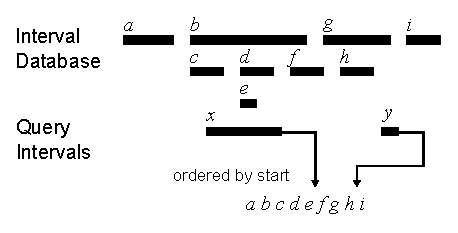
\includegraphics[width=3in]{figures/bits1.eps}
		\label{fig:contained}
		}
		\subfigure[Two lists, one sorted by start and the other by end, can be used to
		find the size of the intersecting set without enumerating the intersecting
		intervals.]{
		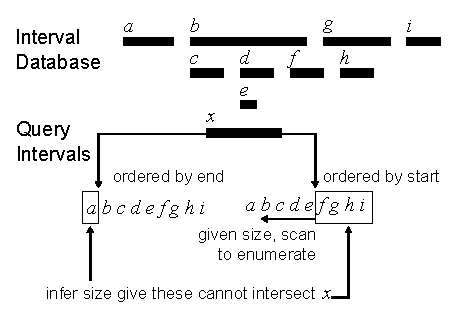
\includegraphics[width=3in]{figures/bits2.eps}
		\label{fig:bits}
		}
		\caption{Contained intervals complicate intersection searches.
		A single list \subref{fig:contained} does not allow for
		efficient searching because all prior intervals must be scanned for
		correctness. Two lists \subref{fig:bits} can be used to
		find the intersecting set size.}
		\label{bitssearching}
	\end{figure}
	

	%%%%%%%%%%%%%%%%%%%%%%%%%%%%%%%%%%%%%%%%%%%%%%%%%%%%%%%%
	% INTRO: Existing methods using alternative strategies
	%%%%%%%%%%%%%%%%%%%%%%%%%%%%%%%%%%%%%%%%%%%%%%%%%%%%%%%%
	\subsection{Existing methods using alternative strategies}

	\textbf{TODO: cite Richardson, BEDTOOLs, BEDOPS}

	Recognizing the limitations of the binary search for detecting interval intersections, several alternative algorithms 
	have been developed that, in general, are either based on trees, NCLists~\citep{alekseyenko2007}, or linear sweeps of 
	pre-sorted intervals~\citep{richardson2006}. The UCSC genome browser introduced a clever and now widely-used 
	scheme based on R-trees. This binning approach partitions intervals from one dataset into hierarchical ``bins''~\citep{kent2002}.  
	Intervals from a second dataset are then compared solely to matching bins (instead of the 
	entire dataset) in order to narrow the search for intersections to a focused portion of the genome.  
	While this popular approach is used by the Kent tools software, BEDTools~\citep{quinlan2010}, 
	SAMTOOLS(\textbf{TODO: cite}), and TABIX(\textbf{TODO: cite}), the underlying tree structure 
	demands substantial memory. 


	%%%%%%%%%%%%%%%%%%%%%%%%%%%%%%%%%%%%%%%%%%%%%%%%%%%%%%%%
	% INTRO: Limits to parallelization
	%%%%%%%%%%%%%%%%%%%%%%%%%%%%%%%%%%%%%%%%%%%%%%%%%%%%%%%%
	\subsection{Limits to parallelization}

	Existing approaches to interval intersection are poor candidates for
	parallelization.  Thread divergence can be a significant problem for
	hierarchical binning methods such as the UCSC binning algorithm.  If intervals
	are not uniformly distributed and a small number of bins contain many intervals
	while other bins are empty, then threads searching full bins will take longer to
	complete than threads searching empty bins.  Since BITS does not enumerate to
	count, interval distribution does not effect divergence.  Binning the 
	hierarchical binning data structure can also be difficult to build in some
	parallel architectures.  For example, in NVIDIA's CUDA at least one extra passes
	over the interval database is required to allocate the correct amount of space 
	for each bin.  BITS uses integer arrays, which easily map to most architectures.

	Recent versions of BEDTools and BEDOPS (\textbf{TODO cite BEDOPS}) conduct a
	linear ``sweep'' through pre-sorted datasets while maintaining an auxiliary
	data structure to track intersections as they are encountered. While the
	complexity of such sequential sweep algorithms is theoretically optimal, the 
	amount of parallelism that exists is limited, and some overhead is required to
	guarantee correctness.  Any linear sweep algorithm must maintain the ``sweep
	invariant''~\cite{mckenney2009}, which states that all segment starts, ends, 
	and intersections behind the sweep must be known.  A parallel sweep algorithm
	must either partition the input space such that each section can be swept in
	parallel without violating the invariant, or threads must communicate 
	about intervals that span partitions.  In the first case parallelism is limited
	to the number of partitions that can be created, and threads can diverge when 
	the number of intervals in each partition are unbalanced.  In the second case,
	the communication overhead between threads prevents the algorithm from being 
	work-effecient and can have significant performance implications.  Several
	parallel sweep algorithms that have been proposed~\citep{goodrich1993,
	kriegel1991, mckenney2009} for segment intersection (a generalization of
	interval intersection), but they all depend on a partitioned input space scheme
	and have limited parallelism and increased overhead.


	% TO DO
	% THIS SHOULD BE MOVED TO THIS CUDA SECTION
	% The current generation of Graphics Processing Units (GPUs), such as NVIDA's
	% CUDA, can improve performance for the subset of problems that map well to the
	% massively parallel single instruction, multiple data (SIMD) architecture. These
	% architectures deploy hundreds of basic parallel processing units, and can
	% support thousands of concurrently executing threads. In order to fully utilize
	% the hardware, a problem must be decomposed into many small subtasks. Problems
	% that do not fit this model are less likely to dramatically benefit from GPU
	% hardware. 
	
	% Search algorithms can expose a higher degree of parallelism by
	% allowing each thread to handle one interval query, making it possible
	% for the parallelism to be proportional to input size, rather than to
	% the distribution of intervals within the input space.  This level of
	% parallelism may not be possible using existing sequential search
	% algorithms, due to their reliance on methods and secondary structures
	% that do not map well onto massively parallel architectures.
	

	



	%%%%%%%%%%%%%%%%%%%%%%%%%%%%%%%%%%%%%%%%%%%%%%%%%%%%%%%%
	% METHODS
	%%%%%%%%%%%%%%%%%%%%%%%%%%%%%%%%%%%%%%%%%%%%%%%%%%%%%%%%
	\section{Methods}
	
	%%%%%%%%%%%%%%%%%%%%%%%%%%%%%%%%%%%%%%%%%%%%%%%%%%%%%%%%
	% METHODS: BITS
	%%%%%%%%%%%%%%%%%%%%%%%%%%%%%%%%%%%%%%%%%%%%%%%%%%%%%%%%
	\subsection{Binary Interval Search (BITS) Algorithm}
	We now introduce our new Binary Interval Search (BITS) algorithm for solving
	the interval set intersection problem.  This algorithm uses binary searches
	to identify interval intersections while avoiding the aforementioned
	complexities caused by contained intervals. The key observation underlying the BITS 
	algorithm is that the size of the intersection between two sets can be 
	determined without \emph{enumerating} each intersection.  For each interval 
	in the query set, two binary searches are performed to determine the \emph{number} 
	of intervals in the database that intersect the query interval.  Each pair of
	searches is independent of all others, and thus all searches can be
	performed in parallel.  
	
	Previously, the intersecting set was defined based on \emph{inclusion}:
	that is, the set of intervals in the interval database $B$ that end after the query
	interval $a_i$ begins, and which begin before $a_i$ ends.  However,
	contained intervals make it difficult to find this set directly.  The
	search for the intersecting intervals can start at the interval in $B$
	closest to $a_i$, but must continue to the beginning of $B$ because
	there is no condition indicating that all intersecting intervals have
	been found.  By restating the intersection definition, we are able to
	determine the size of the intersecting set, which provides a
	terminating condition for the search, so that it may stop once the
	last interval in the intersecting set has been found.

	Our algorithm uses a different, but equivalent, definition of interval
	intersection based on \emph{exclusion}: that is, by identifying the set of 
	intervals in $B$ that \emph{cannot} intersect $a_i$, we can infer how many intervals
	\emph{must} intersect $a_i$. Formally, we define the set of intervals $\mathcal{I}(B,a_i) \in B$ that
	intersect query interval $a_i\in A$ to be the intervals in $B$ that
	are neither in the set of intervals ending before ("left of", set $L$ below) $a_i$ begins,
	nor in the set of intervals starting after ("right of", set $R$ below) $a_i$ ends.  That is:
	\begin{equation*}
		\begin{split}
			\mathcal{L}(B,a_i) = &\{b\in B| b.end < a_i.start\} \\
			\mathcal{R}(B,a_i) = &\{b\in B| b.start > a_i.end\} \\
			\mathcal{I}(B,a_i) = &B / (\mathcal{L}(B,a_i) \cup \mathcal{R}(B,a_i))
		\end{split}
	\end{equation*}

	Finding the intervals in $\mathcal{I}(a_i,B)$ for each $a_i\in A$ by
	taking the difference of $B$ and the union of $\mathcal{L}(B,a_i)$ and
	$\mathcal{G}(B,a_i)$ is not efficient.  However, we can quickly find
	the size of $\mathcal{L}(B,a_i)$ and the size $\mathcal{G}(B,a_i)$,
	then \emph{infer} the size of $\mathcal{I}(B,a_i)$.  With the size of
	$\mathcal{I}(B,a_i)$, we can directly answer the decision problem, the
	counting problem, and the per-interval counting problems.  Moreover,
	the size can also serve as the previously missing (see section 1.1) terminating
	condition in the enumeration problem.

	\begin{algorithm}[h]
		\DontPrintSemicolon
		\footnotesize
		\KwIn{Sorted interval starts and ends $B_S$ and $B_E$, query interval $a$}
		\KwOut{Number of intervals $c$ intersecting $a$}
		\BlankLine
		\textbf{Function} \textsc{ICount}$(B_S,B_E,a)$
		\Begin {
		$first \gets \textsc{BSearch}(B_S, a.end)$\;
		$last \gets \textsc{BSearch}(B_E, a.start)$\;
		$c \gets first - last$\;
		\Return $c$\;
		}
		\caption{Single interval intersection counter}
	\end{algorithm}

	The core function in our algorithm 
	$\textsc{ICount}(B_S,B_E,a_i) = |\mathcal{I}(B,a_i)|$ determines the number of
	intervals in the database $B$ that intersect query interval $a_i$.  As shown in
	Figure~\ref{fig:bits}, $B$ is split into two integer lists 
	$B_S = [b_1.start, b_2.start, \dots, b_M.start]$ and 
	$B_E = [b_1.end, b_2.end, \dots, b_M.end]$, then $B_S$ and $B_E$ are sorted
	numerically.  Next, two binary searches are performed,
	$first=\textsc{ BSearch}(B_S, a_i.end)$ and 
	$last=\textsc{ BSearch}(B_E,
	a_i.start)$.  Since $B_S$ is a sorted list of each interval start coordinate in
	$B$, the elements greater than or equal to $first$ in $B_S$ correspond to the
	set of intervals in $B$ that start after $a_i$ ends.  Similarly, the elements
	less than or equal to $last$ in $B_E$ correspond to the set of intervals in $B$
	that end before $a_i$ starts.  From these two values, we can infer the size of
	the set $\mathcal{I}(B,a_i)$:
	\begin{equation*}
		\begin{split}
			|B|-first=&|\mathcal{R}(B,a_i)| \\
			last=&|\mathcal{L}(B,a_i)| \\ 
			|B|-(last+(|B|-first))=&|\mathcal{I}(B,a_i)|
		\end{split}
	\end{equation*}

	This problem cannot be solved with a single sorted list because
	contained intervals prevent the total ordering of $B$. If $B$ is
	sorted by interval start coordinates, then the interval end
	coordinates may be unordered and $last$ cannot be found
	efficiently.  Similarly, if $B$ is sorted by interval end,
	$first$ can not be found efficiently.  With the subroutine
	$\textsc{ICount}(B_S,B_E,a_i)$ thus defined, the four interval set intersection
	problem variants can now be solved:

	\begin{enumerate}

		\item
		{\em Decision problem:} Let $c$ be an accumulator variable that is
		initialized to zero; then for each $a_i \in A$, accumulate $c = c +
		\textsc{ICount}(B_S,B_E,a_i)$.  If $c\ne0$ then return {\em yes}, otherwise
		return {\em no}.

		\item
		{\em Counting problem:}  Let $c$ be an accumulator variable that is
		initialized to zero; then for each $a_i \in A$, accumulate $c = c +
		\textsc{ICount}(B_S,B_E,a_i)$.  The total accumulated count $c$ is 
		returned (\textbf{Algorithm 2}).

		\item
		{\em Per-interval counting problem:} Let $C$ be an accumulator
		array where element $C[i]$ corresponds to the number of
		intersection for each element in $a_i\in A$.  For each $a_i \in A$,
		set $C[i]=\textsc{ICount}(B_S,B_E,a_i)$.  The total list of counts $C$ is then
		returned (\textbf{Algorithm 3}).

		\item
		{\em Enumeration problem:}
		First find the per-interval counting array $C=\textsc{PerIntervalCounter}(A,B)$
		then the let $R$ be the prefix sum (\textbf{WHAT DOES PREFIX SUM MEAN?)}) of $C$. The array $R$ is used to track the
		number of intervals that must be found in each of the subsequent scans.  Let
		$start = 0$ track the number of enumerated intersections.
		For $i=1\dots|A|$, let $end = R[i]$ where $end - start$ is the number intervals
		in $B$ that intersect $a_i$.  Let $from=\textsc{BSearch}(B_S, a_i.end)$ be
		the initial position of the scan.  While $end - start > 0$ some number of
		intervals in $B$ must be scanned for an intersection with $a_i$.  If $a_i$
		intersections $b_from$ then let $E[start] = <a_i, b_from>$ and 
		$start=start+1$.  Then let $from = from +1$.  Finally, the total set of
		intersecting intervals $E$ is returned (\textbf{Algorithm 4}).
	\end{enumerate}
	
	\begin{algorithm}[h]
		\DontPrintSemicolon
		\footnotesize
		\KwIn{Database intervals array $B$ and query interval array $A$}
		\KwOut{Number of intersections $c$ between $A$ and $B$}
		\BlankLine
		\textbf{Function} \textsc{Counter}$(A,B)$
		\Begin {
		$B_S \gets [b_1.start, \dots, b_M.start]$ where $|B| = M$\;
		$B_E \gets [b_1.end, \dots, b_M.start]$ where $|B| = M$\;
		\textsc{Sort}($B_S$)\;
		\textsc{Sort}($B_E$)\;
		$c \gets 0$\;
		\For{$i \gets 1$ \KwTo $|A|$} {
		$c \gets c + \textsc{ICount}(B_S,B_E,A[i])$
		}
		\Return $c$\;
		}
		\caption{Interval intersection counter}
	\end{algorithm}

	\begin{algorithm}[h]
		\DontPrintSemicolon
		\footnotesize
		\KwIn{Database intervals array $B$ and query intervals array $A$}
		\KwOut{Array of intersections counts $C$ where $|C|=|A|$}
		\BlankLine
		\textbf{Function} \textsc{PerIntervalCounter}$(A,B)$
		\Begin {
		$B_S \gets [b_1.start, \dots, b_M.start]$ where $|B| = M$\;
		$B_E \gets [b_1.end, \dots, b_M.start]$ where $|B| = M$\;
		\textsc{Sort}($B_S$)\;
		\textsc{Sort}($B_E$)\;
		$C \gets [0, \dots, 0]$\;
		\For{$i \gets 1$ \KwTo $|A|$} {
		$C[i] \gets \textsc{ICount}(B_S,B_E,A[i])$
		}
		\Return $C$\;
		}
		\caption{Per interval intersection counter}
	\end{algorithm}

	\begin{algorithm}[h]
		\DontPrintSemicolon
		\footnotesize
		\KwIn{Database intervals array $B$ and query intervals array $A$}
		\KwOut{Array of pair-wise intersections $E$ }
		\BlankLine
		\textbf{Function} \textsc{Enumerator}$(A,B)$
		\Begin {
		$B_S \gets [b_1.start, \dots, b_M.start]$ where $|B| = M$\;
		$B_E \gets [b_1.end, \dots, b_M.start]$ where $|B| = M$\;
		\textsc{Sort}($B_S$)\;
		\textsc{Sort}($B_E$)\;
		$C \gets \textsc{PerIntervalCounter}(A,B)$\;
		$R \gets \textsc{PrefixSum}(C)$\;
		$E \gets [<0,0>, \dots, <0,0>]$\;
		$start \gets 0$\;
		\For{$i \gets 1$ \KwTo $|A|$} {
		$end \gets R[i]$\;
		$from \gets \textsc{BSearch}(B_S, A[i].end)$\;
		\While{$end - start > 0$}{
		\If{ $A[i]$ intersects $B[from]$}{
		$E[start] = <A[i], B[from]>$\;
		$start \gets start + 1$\;
		}		
		$from \gets from - 1$\;
		}
		}
		\Return $E$\;
		}
		\caption{Intersection enumerator}
	\end{algorithm}

	%%%%%%%%%%%%%%%%%%%%%%%%%%%%%%%%%%%%%%%%%%%%%%%%%%%%%%%%
	% METHODS: TIME COMPLEXITY ANALYSIS
	%%%%%%%%%%%%%%%%%%%%%%%%%%%%%%%%%%%%%%%%%%%%%%%%%%%%%%%%
	\subsection{Time Complexity Analysis}
	
	\textbf{DISCUSS THIS SECTION WITH RYAN.  IS IT SUFFICIENT TO PROVE OPTIMALITY?}

	To compute $\textsc{ICount}(B_S,B_E,a_i)$ for each $a_i$ in $A$, the interval
	set $B$ is first split into two sorted integer lists $B_S$ and $B_E$,
	which requires $O(|B| \log |B|)$ time.  Next, each instance of
	$\textsc{ICount}(B_S,B_E,a_i)$ searches both $B_S$ and $B_E$, which consumes
	$O(|A| \log |B|)$ time.  For the counting problems, combining the
	results of all $\textsc{ICount}(B_S,B_E,a_i)$ instances into a final result can
	be accomplished in $O(N)$ time.  The total complexity of the counting
	problems is therefore $O((|A| + |B|) \log |B|)$.
	The enumeration problem requires additional steps to scan the
	intervals in $B_S$.  In the best case scenario, each scan requires
	$\textsc{ICount}(B_S,B_E,a_i)$ extra steps, to a total of $O(|B| \log |B|
	+ C)$ time, where is $C$ is the number of intersections.
	However,
	contained intervals can cause the scan to process more than $C$
	elements.  If there exists some $a_i$ that intersects $b_{j}$ and
	$b_{j-2}$, but not $b_{j-1}$ (i.e., $b_{j-2}$ contains $b_{j-1}$),
	then the enumeration scan will consider one extra element, namely
	$b_{j-1}$.  In the pathological case, $b_0$ contains intervals $\{b_1,
	\dots, b_N\} \in B$, $a_i$ intersects $b_0$, and $a_i$ starts after
	interval $b_N$ ends.  This scenario would cause the enumeration scan
	to consider all the elements in $B$.  If all $a_i$ in $A$ are
	pathological, then each scan would required $|B|$ extra steps, to a
	total of $O(|B| \log |B| + |A||B|)$ time.



	%%%%%%%%%%%%%%%%%%%%%%%%%%%%%%%%%%%%%%%%%%%%%%%%%%%%%%%%
	% RESULTS
	%%%%%%%%%%%%%%%%%%%%%%%%%%%%%%%%%%%%%%%%%%%%%%%%%%%%%%%%
	\section{Results}
	
	%%%%%%%%%%%%%%%%%%%%%%%%%%%%%%%%%%%%%%%%%%%%%%%%%%%%%%%%
	% RESULTS: Performance comparison to existing approaches
	%%%%%%%%%%%%%%%%%%%%%%%%%%%%%%%%%%%%%%%%%%%%%%%%%%%%%%%%
	\subsection{Performance comparison to existing approaches}
	We implemented a single-core version of the BITS algorithm as a C/C++ utility 
	in our BEDTools~\citep{quinlan2010} genome arithmetic suite.
	Here we assess the performance of this sequential BITS implementation to BEDTOOLS and 
	the bedIntersect utility available through the UCSC Genome Browser ("Kent source") \citep{kent2002} 
	(\textbf{see Suppl. Methods - describe commands, how we did timing, what machine, CPU, GPU, startup-time, etc.}).
	We compare the performance of each tool for the \emph{counting}, \emph{per interval counting}, 
	and enumeration problems, as these are the three most widely used interval intersection sub-problems in genomics research. 
	The comparisons presented are based sequence alignment intervals extracted from datasets created 
	for the CEU individual NA12878 by the 1000 Genomes Project\textbf{TO: CITE}).  We randomly sampled 
	between $10^4$ and $10^7$ alignment intervals from both whole-genome and exome-capture datasets for this individual.
	
	Because of the different data structures used, the relative performance of each 
	approach may depend on the genomic distribution of intervals within the sets.  For example, 
	tree-based solutions placing intervals into hierarchical bins may perform poorly when intervals are 
	unevenly distributed among the bins. Therefore, each algorithm was evaluated 
	considering three different interval intersection scenarios:

		\begin{enumerate}
			\item

			{\em Intervals from different distributions} (\textbf{Fig. 2}): the intersection between exome-capture 
			alignments and whole-genome alignments. Since the interval sets have a large number of intervals
			and each set has a different genomic distribution, we expect a small number of intersections.
			
			\item
			{\em Uniform interval distribution} (\textbf{Fig. 3}): the intersection between 
			Refseq exons and genome-wide sequencing data.  Since each interval set
			is, for the most part, evenly distributed throughout the genome, we expect 
			that each exon will intersect roughly the same number of sequencing intervals, 
			and a large number of sequencing intervals will not intersect an exon.

			\item
			{\em Biased interval distribution} (\textbf{Fig. 4}):  the intersection between exons and exome-capture
			alignments.  By design, exome sequencing experiments intentionally bias DNA sequences to the coding exons.  
			Thus, the vast majority of sequence intervals will align in exonic regions. In contrast to the previous 
			scenario, nearly every exon interval will have a large number of sequence interval intersections, and 
			nearly all sequencing intervals will intersect an exon.
		\end{enumerate}

	\subsubsection{BITS excels at counting intersections}
	In all three intersection scenarios, BITS had superior performance for \emph{counting} intersections
	than \emph{enumerating} intersections. This behavior is expected given that design of the BITS algorithm
	is founded upon the observation that, by binary searching the starts and ends of the interval database, 
	intersections can be counted without directly enumerating each intersection. However, recall that in order to enumerate
	intersections (\textbf{Algorithm 4}), BITS must first count the number of intersections and then make 
	a second pass to enumerate each intersection. While enumeration is a limitation of the algorithm, 
	we argue that counting and per interval counting are more relevant to large-scale genomic data exploration. 
	For example, ChIP-seq peak detection proceeds by counting the number of alignments that "pile-up" in focal binding regions \textbf{cite}.
	Similarly, RNAseq analyses use genic read counts to estimate differential expression (\textbf{cite}), and sequence-based 
	approaches for detecting genomic copy-number variation require that the genome is segmented into copy-number states based
	on sequence alignment counts.
	
	\begin{figure}[h]
		\centering
		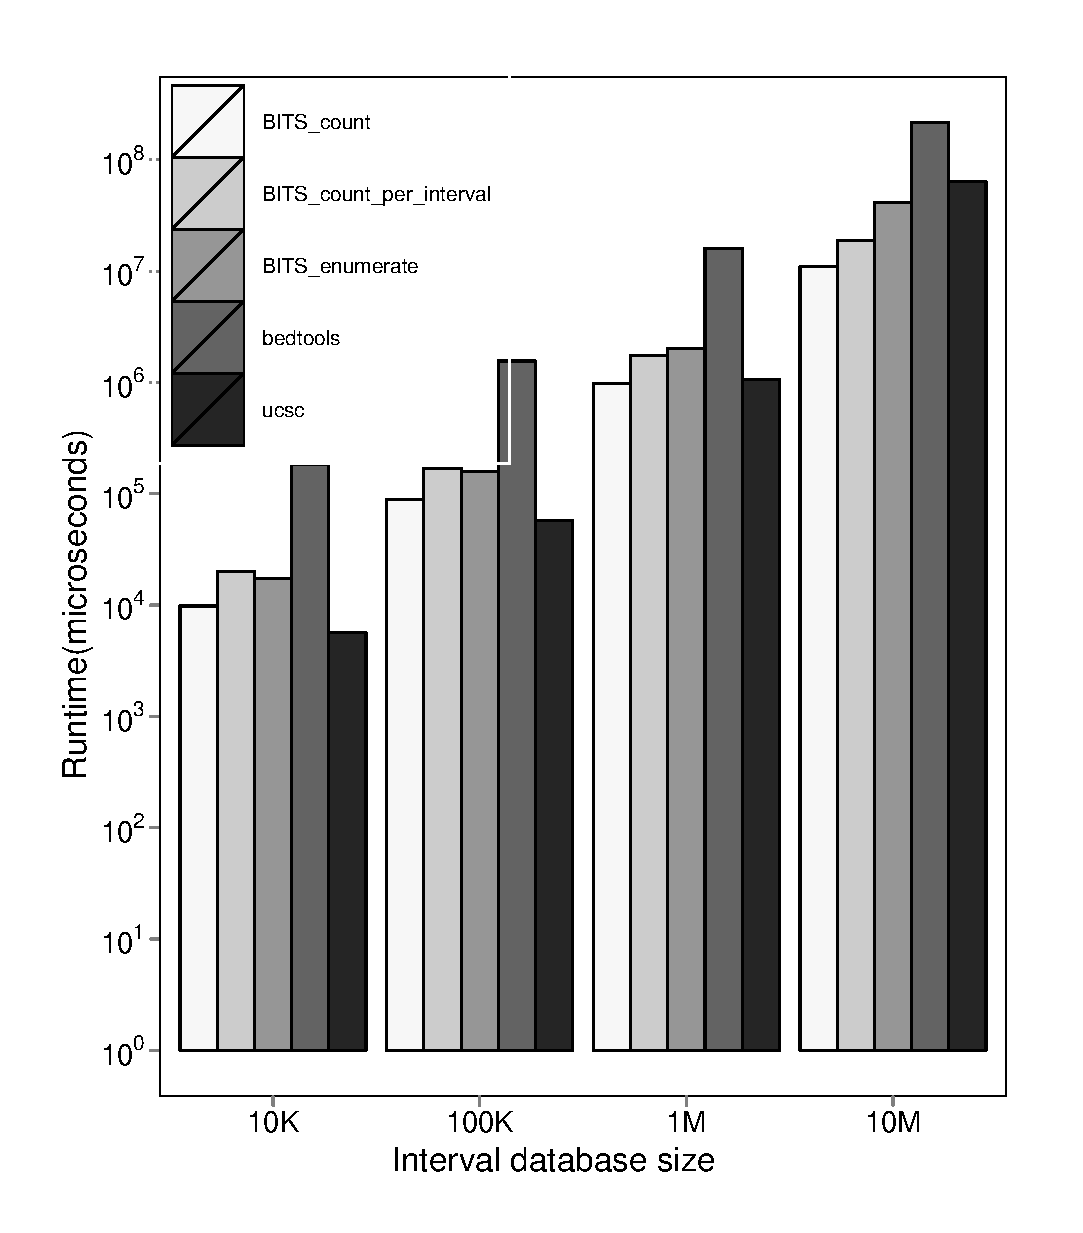
\includegraphics[width=3in]{figures/genome-v-exome.eps}
		\caption[]{Run times for each algorithm using exome and whole-genome datasets (FIX: caption and need error bars).}
	\end{figure}
	
	\subsubsection{BITS is well-suited to large intersections and biased data distributions.}
	While our BITS implementation substantially (between X and Y times faster) outperformed BEDTOOLS 
	in all scenarios, it was, on average, X \textbf{fix me!} times slower than the UCSC bedIntersect utility. 
	In part, this may be due to the maturity and technical sophistication of the Kent source tools. However, the
	primary contribution is likely the fundamental differences in the data structures used by
	the UCSC binning algorithm and by BITS.  The UCSC binning algorithm distributes genomic intervals
	into hierarchical bins, and as such, excels when intervals are evenly distributed among bins, \emph{and}
	when individual bins contain a relatively small number of intervals.  However, the performance of the algorithm
	is diminished for very large datasets, even when the intervals are evenly distributed, as on average, the number
	of intervals in each queried bin will be relatively large (\textbf{Fig. 2}; size = 1e7). In contrast, as BITS is based on
	binary search ($O(\log |B|)$ complexity), its performance scales more linearly with respect to dataset size.

	
	Similarly, datasets such as exome-capture experiments lead to biased distributions of intervals among the UCSC bins.
	Consequently, most bins contain no intervals, while a small fraction contain many intervals. When the query intervals
	reflect the same bias, the overhead of the UCSC algorithm is more onerous, as a small number of bins are queried 
	and each queried bin contains many intersecting intervals that must be enumerated. As the BITS algorithm
	is agnostic to the interval distributions, it will outperform the UCSC algorithm for common genomic analyses such
	as ChIP-seq, RNA-seq, and CNV detection, especially for the typically large sequence alignment datasets
	that these experiments generate ((\textbf{Fig. 4})).
	
	\begin{figure}[h]
		\centering
		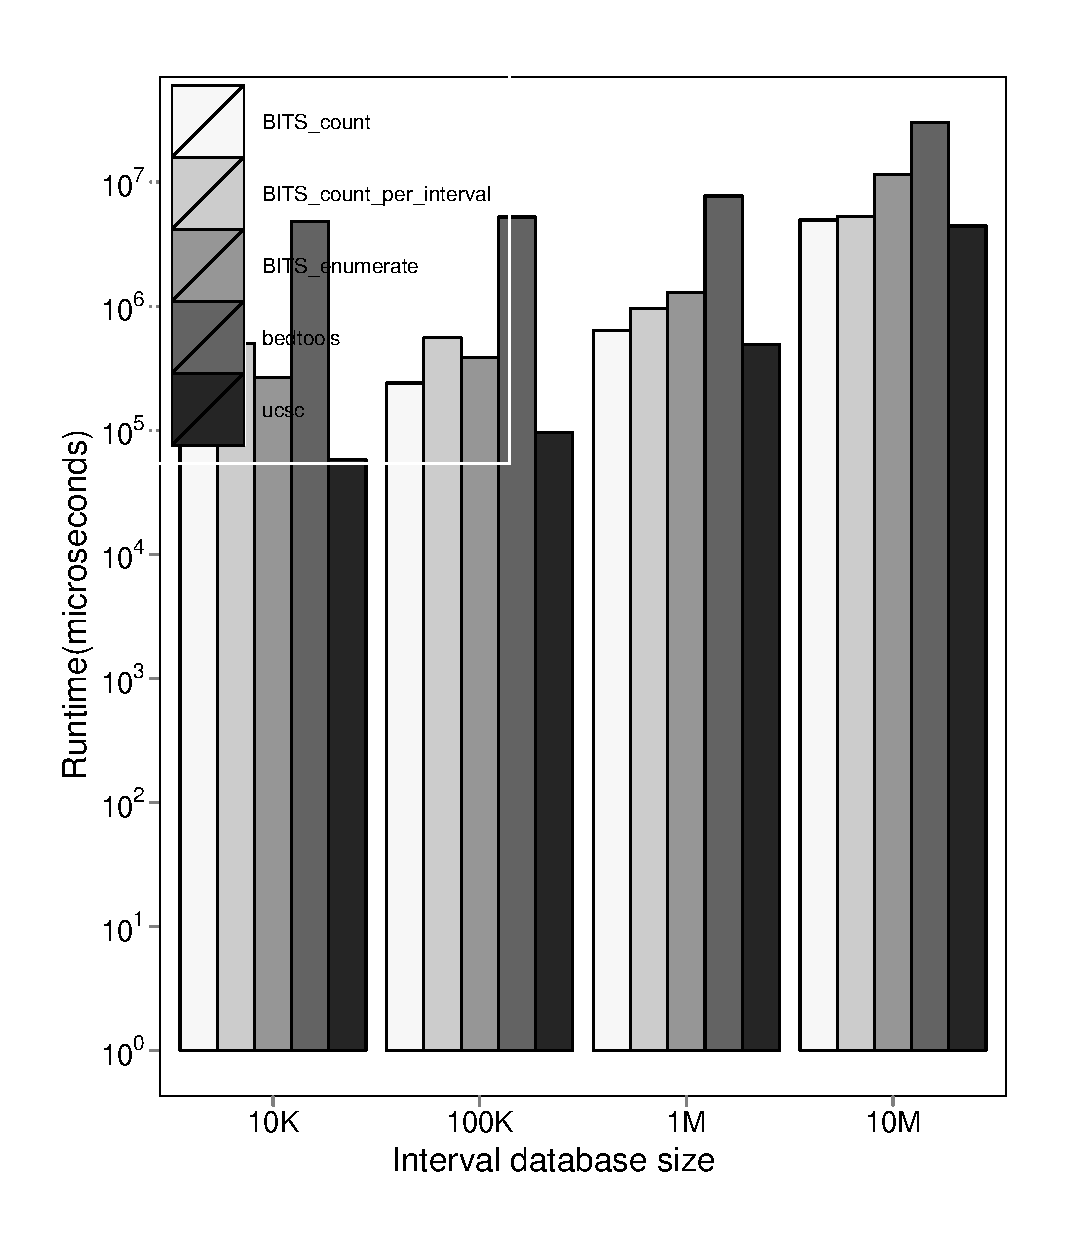
\includegraphics[width=3in]{figures/exons-v-genome.eps}
		\caption[]{Run times for each algorithm using exons and whole-genome datasets (FIX: caption and need error bars).}
	\end{figure}
	
	
	\begin{figure}[h]
		\centering
		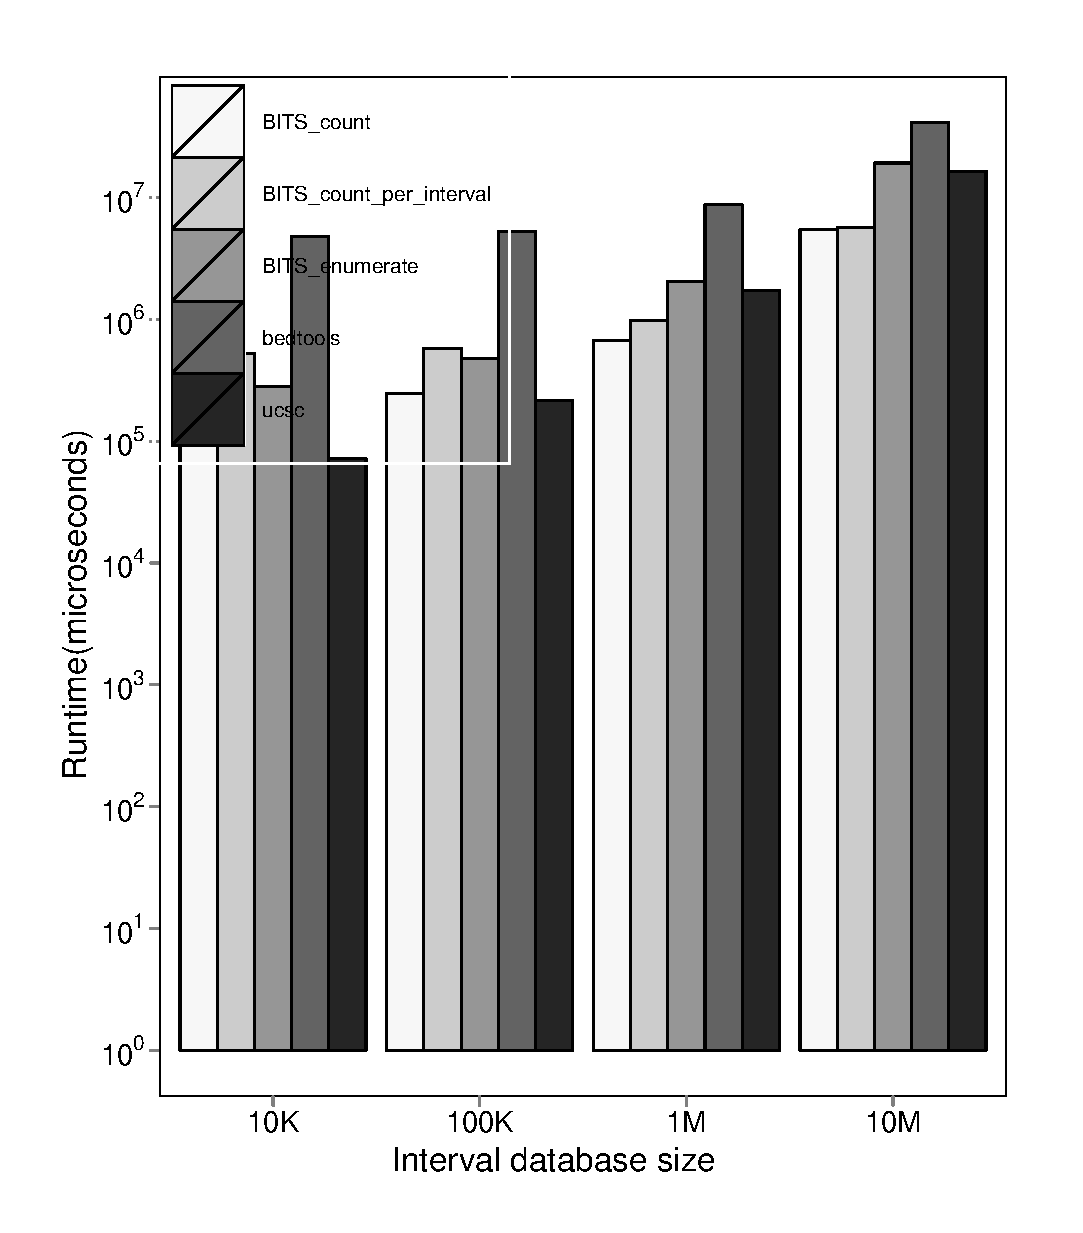
\includegraphics[width=3in]{figures/exons-v-exome.eps}
		\caption[]{Run times for each algorithm using exons and whole-exome datasets (FIX: caption and need error bars).}
	\end{figure}
	
	% the primary functions used to analyze large data sets.  For
	% example, the utility of the full list of 9,148,823 intersection between human
	% exon and the exome sequencing of the NA12878 individual (the biased distribution
	% scenario) is limited, while the number of intersections per exon can provide
	% insight into deletions, duplications, and other properties of NA12878's
	% genome.
	% 
	% The performance profiles of counting (Figure~\ref{count}) and per interval
	% counting (Figure~\ref{perintervalcount}) were similar for all algorithms.
	% In these two scenarios, excluding the smallest data sets, all versions of BITS
	% performed faster than both Kent tools and BEDTools.  For the 10K database, Kent
	% tools performed faster than the sequential and OpenMP version of BITS by up to a
	% factor of three.  The following table gives the average speedups of the three
	% versions of BITS over Kent tools and BEDTools for the 10 million interval
	% database.
	% 
	% For enumeration, the performance improvements of the  sequential and OpenMP
	% versions of BITS were an order of magnitude lower against BEDTools, and
	% non-existent against Kent tools.  In fact, Kent tools performed better than
	% sequential BITS by a factor of nearly three for the smallest database
	% (Figure~\ref{fig:eexonfull}), and the run times of the two where nearly
	% equivalent for the largest database.  The CUDA version of BITS did provide a
	% modest improvement over both Kent tools and BEDTools, but at a level lower than
	% in counting and per interval counting.
	% The following table  gives the average speedups of the three versions of BITS
	% over Kent tools and BEDTools for the 10 million interval database.
	% All run-times were measured on a 2.66 GHz quad-core Intel Xeon X555 CPU with 8
	% MB of cache running Ubuntu Linux version 4.4.3 (kernel version 2.6.32-34).
	% Run-times for CUDA were measured on an NVIDIA Tesla C2050 GPU with 448 1.15 GHz
	% cores, 3 GB of global memory, CUDA driver version 4246739, and CUDA runtime
	% version 4.0.  The source code was compiled using gcc version 4.4.3, and NVIDIA
	% CUDA compilation tools release 4.0, V0.2.1221.  In each case, run-times measure 
	% the performance of the intersection algorithm and thus do not include disk
	% reading, writing, or the time required to initialize the GPU.

	% The results of our tests are given in Figure~\ref{count},
	% Figure~\ref{perintervalcount}, and Figure~\ref{enumerate}.
	
	
	% In nearly every case, the sequential version of BITS outperformed both Kent
	% tools and BEDTools.  The most striking improvement was in the interval counting
	% operation, where ---in the largest operation (10M many short intervals, a total
	% of 2e$^7$ intervals)--- sequential BITS achieved a speedup of 7.7x over Kent
	% tools and 27.4x over BEDTools.  In this same case the speedup over Kent tools
	% and BEDTools by OpenMP BITS was 13.1x and 46.6x, and the speedup by CUDA BITS
	% was 143.7x and 508.8x, respectively.
	% 
	% While BITS did have some improvement in enumeration operation, the speedup was
	% an order of magnitude lower than in the counting operations, and Kent tools
	% performed better than sequential bits in one scenario.  This result is expected
	% given that BITS is optimized for counting intersections, which is generally more
	% a useful operation in large-scale comparisons.

	%\begin{table}[h]
	%\caption{Average speedup for intersection counting and per interval counting for
	%the 10M database}
	%\centering
	% \begin{center}
	% 	\begin{tabular}{lll}
	% 		\\
	% 		& Kent tools & BEDTools \\
	% 		\hline
	% 		Sequential	& 4.5x	& 17.7x \\
	% 		OpenMP		& 11.1x	& 43.1x \\
	% 		CUDA		& 75.8x	& 285.4x \\
	% 		\\
	% 	\end{tabular}
	% \end{center}
	%\label{table:avgcp}
	%\end{table}

	%\begin{table}[h]
	%\caption{Average speedup for intersection enumeration for the 10M database.}
	%\centering
	% \begin{center}
	% 	\begin{tabular}{lll}
	% 		\\
	% 		& Kent tools & BEDTools \\
	% 		\hline
	% 		Sequential	& 1.5x & 7.3x \\
	% 		OpenMP		& 1.3x & 6.4x \\
	% 		CUDA		& 3.8x & 24.9x \\
	% 		\\
	% 	\end{tabular}
	% \end{center}
	%\label{table:avge}
	%\end{table}


	%%%%%%%%%%%%%%%%%%%%%%%%%%%%%%%%%%%%%%%%%%%%%%%%%%%%%%%%
	% RESULTS: Parallel implementations 
	%%%%%%%%%%%%%%%%%%%%%%%%%%%%%%%%%%%%%%%%%%%%%%%%%%%%%%%%
	\subsection{Parallel implementations}
	
	As we have demonstrated, the BITS algorithm is well-suited to counting
	interval intersections, regardless of dataset size or genomic distribution.
	
	\begin{enumerate}
		\item Simple data structure - array.
		\item Binary search - O(log(N))
		\item these make it easily portable to parallel architectures, even 
		      more complicated archs such as CUDA.
		\item we implemented BITS for OpenMP and CUDA (supp. methods).
		\item describe scaleups.
		\item GPUs - sort, arrays, bsearch.  all things GPUs excel at.
	\end{enumerate}	
	
	\begin{table}[h]
	\centering
	\begin{center}
		\begin{tabular}{l l l l l l}
			Arch. & Size & Total & Intersection & I/O & Speedup \\
			\hline
			\hline
			OpenMP & 10K & 102,769 & 26.7\% & 73.4\% & 1.85 \\
			OpenMP & 100K & 129,344 & 29.4\% & 70.6\% & 1.90 \\
			OpenMP & 1M & 391,332 & 36.4\% & 63.6\% & 1.71 \\
			OpenMP & 10M & 3,352,776 & 44.0\% & 56.0\% & 1.63 \\ 
			\\
			CUDA & 10K & 86,521 & 10.0\% & 90.0\% & 2.21 \\
			CUDA & 100K & 104,697 & 10.3\% & 89.7\% & 2.34 \\
			CUDA & 1M & 272,418 & 8.6\% & 91.4\% & 2.45 \\
			CUDA & 10M & 2,028,921 & 7.1\% & 92.9\% & 2.70 \\
			\\
		\end{tabular}
	\end{center}
	\label{table:avge}
	\caption{Average speed and scaleup over sequential algorithm for the counting problem on exons v. exome.}
	\end{table}
	
	
	% Performing a single operation independently on many different inputs
	% is a classic parallelization scenario.  When based on the subroutine
	% $\textsc{ICount}(B_S,B_E,a_i)$, which is independent of all 
	% $\textsc{ICount}(B_S,B_E,a_j)$
	% for $a_j \in A$ where $i \neq j$, interval set intersection can be a
	% {\em pleasingly parallelizable} problem that easily maps to a number
	% of parallel architectures.
	% 
	% \subsubsection{OpenMP}
	% 
	% A popular option for parallelizing applications is the OpenMP standard.
	% Converting a sequential program into a parallel program can be as simple as
	% adding a single compiler directive.  We report performance benchmarks using
	% OpenMP as a comparison reference when considering alternative parallel
	% architectures.
	% 
	% \subsubsection{CUDA}
	% 
	% NVIDIA's Compute Unified Device Architecture (CUDA) is a single
	% instruction multiple data (SIMD) architecture that provides
	% programmers a general interface to a large number of parallel graphics
	% processing units (GPUs).
	% 
	% The BITS algorithm is especially well suited for the NVIDIA CUDA
	% architecture for a number of reasons.  First, CUDA is optimized to handle large
	% numbers of threads.  By assigning each thread one instance of
	% $\textsc{ICount}(B_S,B_E,a_i)$ for all $a_i \in A$, the number of threads will
	% be proportional to the file size.  CUDA threads also execute in lock-step and
	% any divergence between threads will cause reduced thread utilization.  While
	% there is some divergence in the depth of each binary search performed by
	% $\textsc{ICount}(B_S,B_E,a_i)$, it has an upper bound of $O(log |B|)$.  Outside of
	% this divergence $\textsc{ICount}(B_S,B_E,a_i)$ is a classic SIMD operation.  And
	% finally, the only data structure required for this algorithm is a sorted list.
	% Sorting on GPU has been an active area of research for many years, and current
	% GPU sorting algorithms can sort billions of integers within
	% seconds~\citep{merrill2011}.
	% 
	% 
	% While BITS maps well to multiple parallel architectures (multi-core CPU using OpenMP,
	% and NVIDIA GPU using CUDA), a fair comparison cannot be made between parallel
	% BITS and Kent tools or BEDTools because parallel version of these packages are
	% not available.  Therefore, we demonstrate the value of our algorithm by
	% comparing sequential versions.  We then show the added benefit provided by 
	% BITS using parallel architectures.
	
	

	%%%%%%%%%%%%%%%%%%%%%%%%%%%%%%%%%%%%%%%%%%%%%%%%%%%%%%%%
	% RESULTS: Applications for Monte-carlo simulations 
	%%%%%%%%%%%%%%%%%%%%%%%%%%%%%%%%%%%%%%%%%%%%%%%%%%%%%%%%
	\subsection{Applications for Monte-carlo simulations}
	

	

	%%%%%%%%%%%%%%%%%%%%%%%%%%%%%%%%%%%%%%%%%%%%%%%%%%%%%%%%
	% CONCLUSION
	%%%%%%%%%%%%%%%%%%%%%%%%%%%%%%%%%%%%%%%%%%%%%%%%%%%%%%%%
	\section{Conclusion}
	
	We have devised a scalable new approach to interval intersection
	that exploits the simplicity of the binary search while avoiding the complications
	posed by nested intervals. Our binary interval search (BITS) algorithm is founded upon the novel 
	observation that the count of overlapping intervals between two sets 
	can inferred by using binary searches to identify intervals that \emph{cannot}
	intersect one another. Unlike existing methods, our approach does not need
	to enumerating each individual intersection in order to count the total number 
	of intersections. We have demonstrated that, when implemented using a single process,
	BITS compares favorably to existing tools and excels at intersection counting, especially
	for very large datasets (e.g., high throughput sequencing) or datasets with biased
	genomic distributions (e.g., ChIP-seq, exome capture, RNA-seq).
	
	We also show that the two binary searches conducted
	against the database for each query interval are independent, and thus, parallelizable.
	This property, combined with the simple data structures and search algorithms employed
	make the BITS algorithm a perfect candidate for GPU architectures that are optimized for
	large numbers of concurrent threads. Our results with the CUDA architecture
	demonstrate speed increases of up to ?x and ?x relative to existing 
	approaches to genome interval intersection. This substantial performance increase 
	is especially relevant to modern genomic analyses given the staggering scale and complexity 
	of current and future datasets.  Given that the BITS algorithm excels at \emph{counting}
	overlaps, it is perfectly suited to address many fundamental yet computationally
	intensive genomic analyses including RNA-seq transcript quantification, ChIP-seq
	peak detection, and searches for copy-number and structural variation.
	
	\textbf{TO DO: Discuss MCMC.}
	
	\textbf{TO DO: Discuss more performant versions when data is pre-sorted.}

	\textbf{TO DO: Discuss the potential for using BITS for new statistical measures.  For
	example, the Jaccard measure in the recent PLoS CompBio paper.}
	
	Given the performance and simplicity of the algorithm, we
	anticipate that it will benefit a wide range of existing tools ranging from
	visualization tools to widely-used genomic analysis software.

	\bibliographystyle{natbib}
	%\bibliographystyle{achemnat}
	%\bibliographystyle{plainnat}
	%\bibliographystyle{abbrv}
	%\bibliographystyle{bioinformatics}
	%
	%\bibliographystyle{plain}
	%
	\bibliography{bioinformatics}
\end{document}
